% Copyright 2004 by Till Tantau <tantau@users.sourceforge.net>.
%
% In principle, this file can be redistributed and/or modified under
% the terms of the GNU Public License, version 2.
%
% However, this file is supposed to be a template to be modified
% for your own needs. For this reason, if you use this file as a
% template and not specifically distribute it as part of a another
% package/program, I grant the extra permission to freely copy and
% modify this file as you see fit and even to delete this copyright
% notice. 

\documentclass{beamer}

% There are many different themes available for Beamer. A comprehensive
% list with examples is given here:
% http://deic.uab.es/~iblanes/beamer_gallery/index_by_theme.html
% You can uncomment the themes below if you would like to use a different
% one:
%\usetheme{AnnArbor}
%\usetheme{Antibes}
%\usetheme{Bergen}
%\usetheme{Berkeley}
%\usetheme{Berlin}
%\usetheme{Boadilla}
%\usetheme{boxes}
%\usetheme{CambridgeUS}
%\usetheme{Copenhagen}
%\usetheme{Darmstadt}
%\usetheme{default}
%\usetheme{Frankfurt}
%\usetheme{Goettingen}
%\usetheme{Hannover}
%\usetheme{Ilmenau}
%\usetheme{JuanLesPins}
%\usetheme{Luebeck}
\usetheme{Madrid}
%\usetheme{Malmoe}
%\usetheme{Marburg}
%\usetheme{Montpellier}
%\usetheme{PaloAlto}
%\usetheme{Pittsburgh}
%\usetheme{Rochester}
%\usetheme{Singapore}
%\usetheme{Szeged}
%\usetheme{Warsaw}


% Customize Warsaw color 
\setbeamercolor*{palette primary}{use=structure,fg=white,bg=red!50!black}
\setbeamercolor*{palette secondary}{use=structure,fg=white,bg=red!60!black}
\setbeamercolor*{palette tertiary}{use=structure,fg=white,bg=red!70!black}

% Customize Warsaw block title and background colors
\setbeamercolor{block title}{bg=red!50!black,fg=white}


% List your packages here

\usepackage[colorinlistoftodos]{todonotes}
\usepackage{caption}

\title[BEMOSS Installation]{BEMOSS and Its Enhanced Applications}

% % A subtitle is optional and this may be deleted
% \subtitle{Product Proposal}

\author[B.~Lauer]{Brian~Lauer \\\and
Advisor: Dr. Suruz Miah}
% - Give the names in the same order as the appear in the paper.
% - Use the \inst{?} command only if the authors have different
%   affiliation.

\institute[Bradley University] % (optional, but mostly needed)
{
  Department of Electrical and Computer Engineering\\
  Bradley University\\
  1501 W. Bradley Avenue\\
  Peoria, IL, 61625, USA
}
% - Use the \inst command only if there are several affiliations.
% - Keep it simple, no one is interested in your street address.

\date[June~21,~2019]{Friday, June~21,~2019}
% - Either use conference name or its abbreviation.
% - Not really informative to the audience, more for people (including
%   yourself) who are reading the slides online

\logo{\hfill\href{http://www.bradley.edu}{
\includegraphics[width=0.75cm]{figs/logoBU1-Print}}}  % place logo in every page 


\subject{Mobile Robot Localization}
% This is only inserted into the PDF information catalog. Can be left
% out. 

% If you have a file called "university-logo-filename.xxx", where xxx
% is a graphic format that can be processed by latex or pdflatex,
% resp., then you can add a logo as follows:

% \pgfdeclareimage[height=0.5cm]{university-logo}{university-logo-filename}
% \logo{\pgfuseimage{university-logo}}

% Delete this, if you do not want the table of contents to pop up at
% the beginning of each subsection:
% \AtBeginSubsection[]
% {
% \begin{frame}<beamer>{Outline}
%   \tableofcontents[currentsection,currentsubsection]
% \end{frame}
% }

% Let's get started
\begin{document}

\begin{frame}
  \titlepage
\end{frame}

\begin{frame}{Outline}
  \tableofcontents
  % You might wish to add the option [pausesections]
\end{frame}

% Section and subsections will appear in the presentation overview
% and table of contents.
%----------------------------------

\section{Install Ubuntu 16.04}
\subsection{On Disk}
\begin{frame}{Install Ubuntu 16.04}{On Disk}
	\begin{columns}[T]
		\begin{column}{0.5\textwidth}
			\begin{figure}
				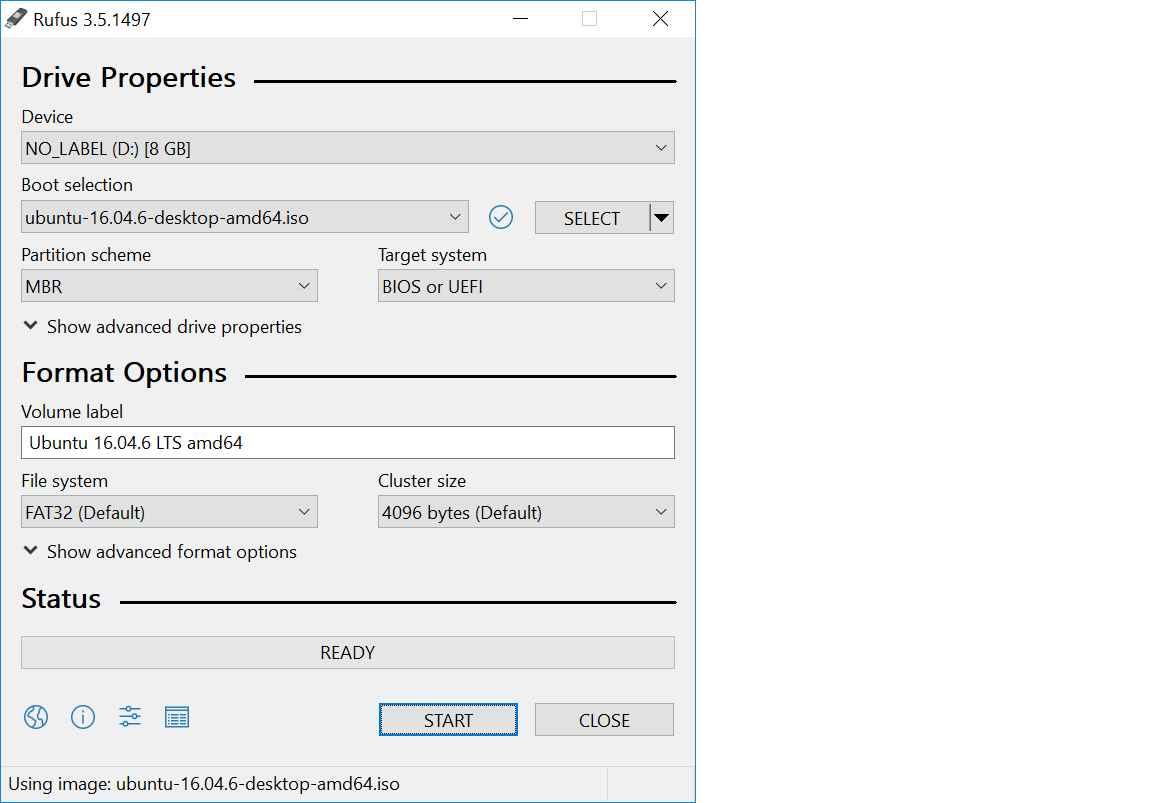
\includegraphics[scale=0.17]{figs/rufus_en_2x.png}
				\caption{Rufus USB Formatting Utility}
			\end{figure}
			\begin{figure}
				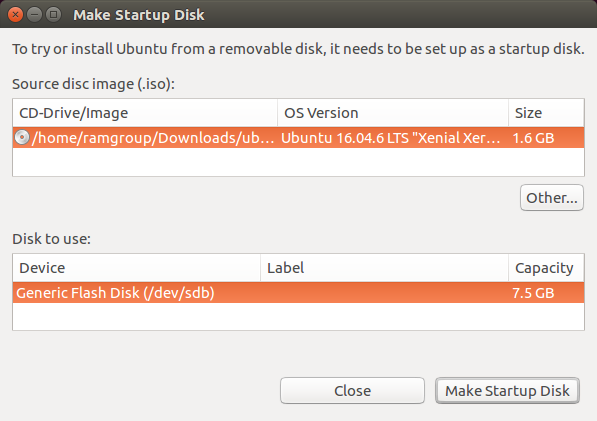
\includegraphics[scale=0.15]{figs/startupDiskCreator.png}
				\caption{Startup Disk Creator}
			\end{figure}
		\end{column}
		\begin{column}{0.5\textwidth}
			\begin{block}{Link}
				\url{http://releases.ubuntu.com/16.04/}
			\end{block}
			\begin{block}{Create Bootable Flash Medium}
			\begin{itemize}
				\item Rufus (Windows)
				\item SanDisk Cruzer Media (MacOS)
				\item Startup Disk Creator (Linux)
			\end{itemize}
			\end{block}
		\end{column}
	\end{columns}	  
\end{frame}

%----------------------------------

\subsection{Virtual Machine}

\begin{frame}{Install Ubuntu 16.04}{Virtual Machine}
	\begin{columns}[T]
		\begin{column}{0.5\textwidth}
			\begin{figure}
				\centering
				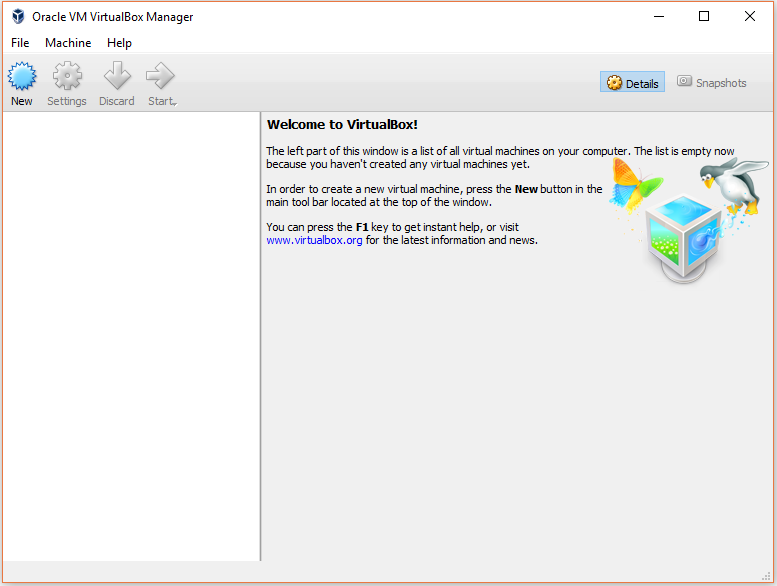
\includegraphics[scale=0.26]{figs/mainpage_virtualbox.png}
				\caption{Oracle VM VirtualBox Manager, 
				courtesy of https://github.com/bemoss/wiki\_images/}
			\end{figure}
		\end{column}
		\begin{column}{0.5\textwidth}
			\begin{block}{Links}
				\begin{enumerate}
					\item https://www.virtualbox.org/
					wiki/Downloads
					\item https://github.com/bemoss/
					BEMOSS3.5/wiki/Ubuntu-Installation
				\end{enumerate}
			\end{block}
		\end{column}
	\end{columns}
\end{frame}

%----------------------------------

\section{Install BEMOSS Launcher Wizard}

\begin{frame}{Install BEMOSS Launcher Wizard}{}
\begin{columns}[T]
	\begin{column}{0.5\textwidth}
		\begin{figure}
			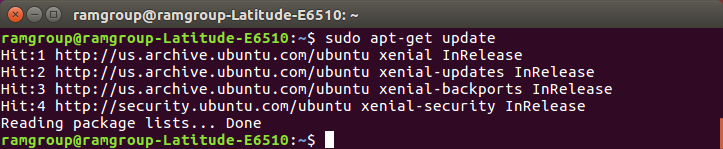
\includegraphics[scale=0.2]{figs/aptgetUpdate.png}
			\caption{Updating the system}
		\end{figure}
		\begin{figure}
			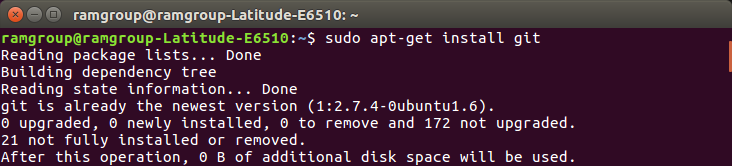
\includegraphics[scale=0.2]{figs/installgit.png}
			\caption{Installing git}
		\end{figure}
		\begin{figure}
			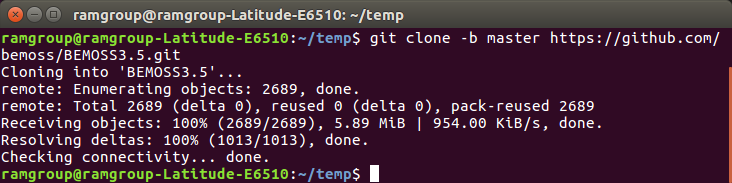
\includegraphics[scale=0.2]{figs/clonebemoss.png}
			\caption{Cloning BEMOSS}
		\end{figure}
	\end{column}	
	\begin{column}{0.5\textwidth}
		\begin{block}{Steps}
			\begin{enumerate}
				\item Open a terminal
				\item Update the system
				\item Install git
				\item Clone BEMOSS repo
			\end{enumerate}
		\end{block}
	\end{column}
\end{columns}
\end{frame}

%----------------------------------

\section{Launch BEMOSS Launcher Wizard}

\begin{frame}{Launch BEMOSS Launcher Wizard}
\begin{columns}[T]
	\begin{column}{0.5\textwidth}
		\begin{figure}
			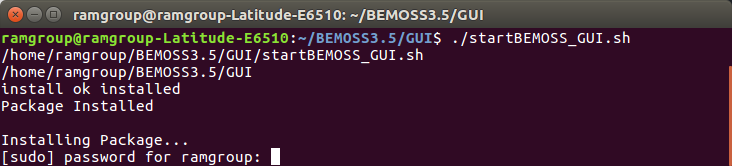
\includegraphics[scale=0.2]{figs/startBEMOSSrelative.png}
			\caption{Running \texttt{startBEMOSS\_GUI.sh} using a relative path}
		\end{figure}
		\begin{figure}
			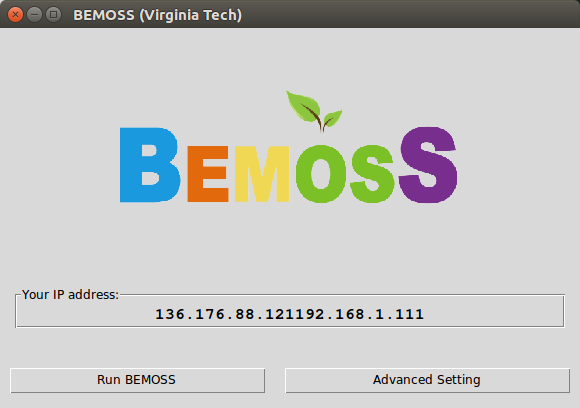
\includegraphics[scale=0.2]{figs/bemossWizard.png}
			\caption{BEMOSS Launcher Wizard}
		\end{figure}
	\end{column}
	\begin{column}{0.5\textwidth}
		\begin{block}{Steps}
			\begin{enumerate}
				\item Run \texttt{startBEMOSS\_GUI.sh} in \texttt{/\#bemoss\_folder/
				BEMOSS3.5/GUI}
				\item Enter system password
			\end{enumerate}
		\end{block}
	\end{column}		
\end{columns}
\end{frame}

\section{Install BEMOSS System}

\begin{frame}{Install BEMOSS System}
\begin{columns}[T]
	\begin{column}{0.5\textwidth}
		\begin{figure}
			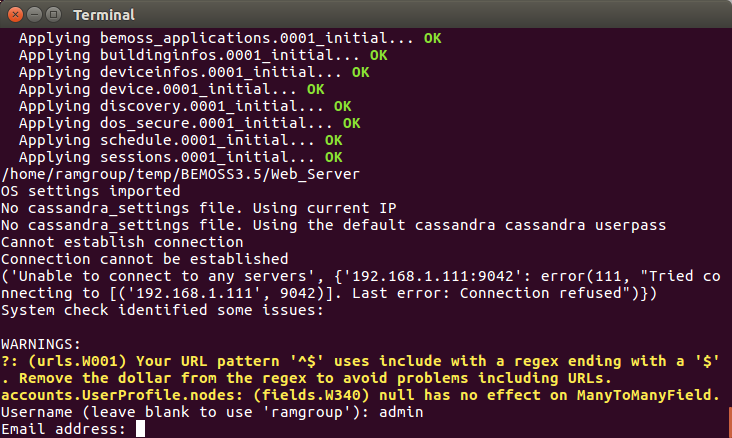
\includegraphics[scale=0.15]{figs/djangoSuperuser.png}
			\caption{Prompt for Django Superuser}
		\end{figure}
		\begin{figure}
			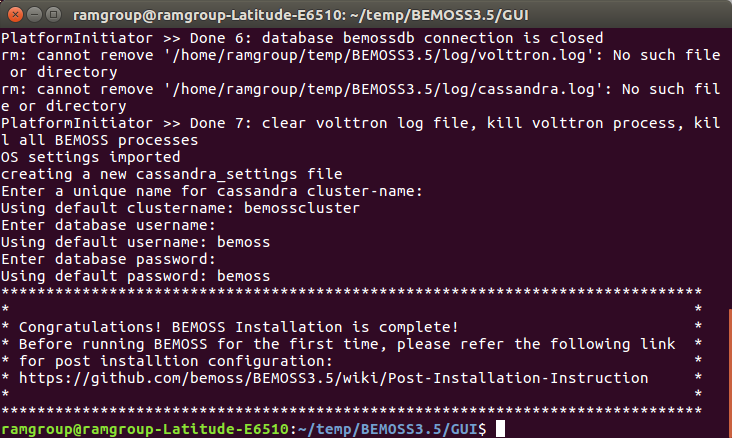
\includegraphics[scale=0.15]{figs/bemossFinish.png}
			\caption{Cassandra database login info}
		\end{figure}
	\end{column}
	\begin{column}{0.5\textwidth}
		\begin{block}{Steps}
			\begin{enumerate}
				\item Click "Run BEMOSS"
				\item Define Django Superuser
				\item Define parameters for Cassandra database
			\end{enumerate}
		\end{block}
	\end{column}
\end{columns}
\end{frame}

\section{Post-Installation}

\subsection{Configure PostgreSQL database}
\begin{frame}{Post-Installation}{Configure PostgreSQL database}
\begin{columns}[T]
	\begin{column}{0.5\textwidth}
		% advanced settings figure
		\begin{figure}
			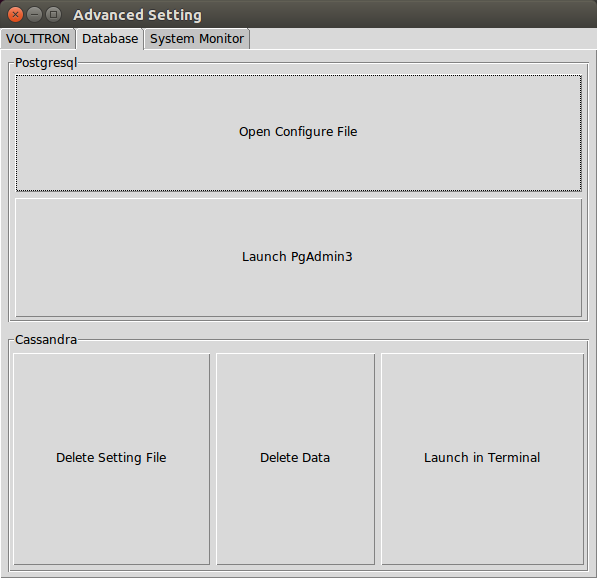
\includegraphics[scale=0.2]{figs/advancedSettings.png}
			\caption{Advanced Settings window}
		\end{figure}
	\end{column}
	\begin{column}{0.5\textwidth}
		\begin{block}{Steps}
			\begin{enumerate}	
				\item Click "Advanced Setting"
			\end{enumerate}		
		\end{block}
	\end{column}
\end{columns}
\end{frame}

\begin{frame}{Post-Installation}{Configure PostgreSQL database}
\begin{columns}[T]
\begin{column}{0.5\textwidth}
	\begin{figure}
		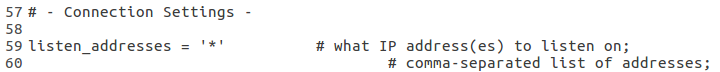
\includegraphics[scale=0.2]{figs/postgresqlChange.png}
		\caption{\texttt{postgresql.conf} lines 57-60}
	\end{figure}
	\begin{figure}
		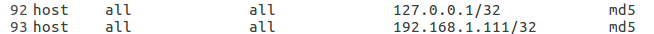
\includegraphics[scale=0.2]{figs/pg_hbaChange.png}
		\caption{\texttt{pg\_hba.conf} lines 92-93}
	\end{figure}
\end{column}
\begin{column}{0.5\textwidth}
	\begin{block}{Steps (Cont.)}
		\begin{enumerate}
			\setcounter{enumi}{1}
			\item Change line 59 of \texttt{postgresql.conf} to \texttt{listen\_addresses = '*'}

			\item Copy line 92 of \texttt{pg\_hba.conf} and paste on line 93
			\item Change IP address on line 93 to system's IP address
		\end{enumerate}
	\end{block}		
\end{column}
\end{columns}
\end{frame}

\begin{frame}{Post-Installation}
	\begin{columns}[T]
		\begin{column}{0.5\textwidth}
			\begin{figure}
				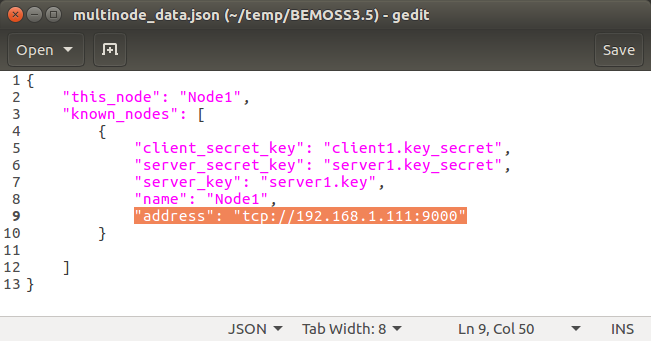
\includegraphics[scale=0.2]{figs/multinodeChange.png}
				\caption{\texttt{multinode\_data.json} open in gedit}
			\end{figure}
			\begin{figure}
				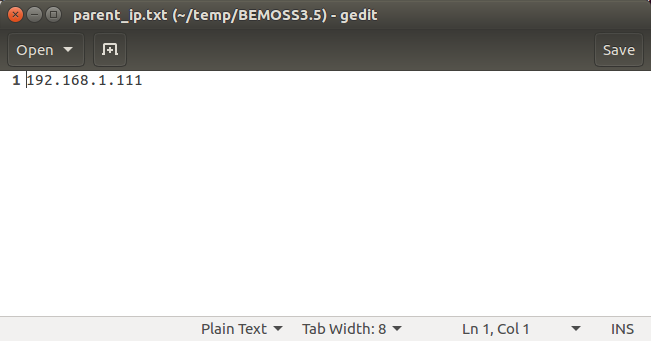
\includegraphics[scale=0.2]{figs/parentipChange.png}
				\caption{parent\_ip.txt open in gedit}
			\end{figure}
		\end{column}
		\begin{column}{0.5\textwidth}
			\begin{block}{Steps (Cont.)}
				\begin{enumerate}
					\setcounter{enumi}{4}
					\item Modify \texttt{multinode\_data.json} in \texttt{/\#bemoss\_folder/BEMOSS3.5} with system's IP address
					\item Modify \texttt{parent\_ip.txt} in \texttt{/\#bemoss\_folder/BEMOSS3.5} with system's IP address
				\end{enumerate}
			\end{block}
		\end{column}
	\end{columns}
\end{frame}

\section{Problems}

\begin{frame}{Problems}
	\begin{columns}[T]
		\begin{column}{0.5\textwidth}
			\begin{figure}
				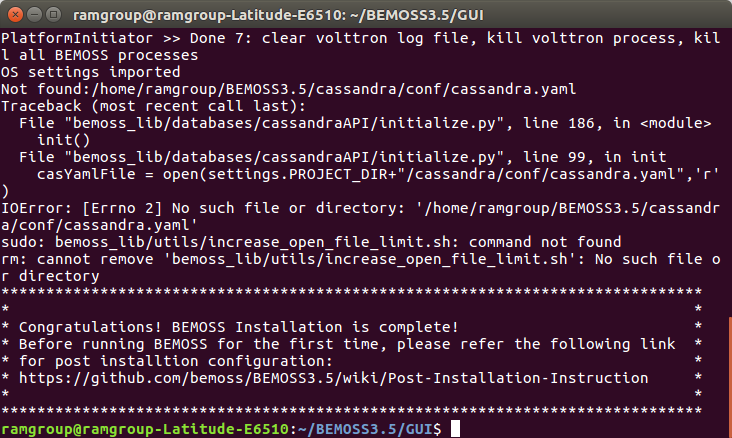
\includegraphics[scale=0.2]{figs/screenshot61019.png}
				\caption{Error raised by BEMOSS during installation}
			\end{figure}
			\begin{figure}
				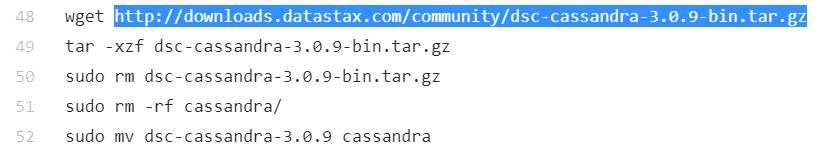
\includegraphics[scale=0.4]{figs/datastaxURLError.png}
				\caption{Lines 48-52 of \texttt{bemoss\_install\_v3.5.sh}}
			\end{figure}
		\end{column}
		\begin{column}{0.5\textwidth}
			\begin{block}{Description}
				\begin{itemize}
					\item Cassandra directory non-existant
					\item Broken link on line 48 of \texttt{bemoss\_install\_v3.5.sh} in \texttt{/\#bemoss\_folder/
					BEMOSS3.5/GUI}
				\end{itemize}
			\end{block}
		\end{column}
	\end{columns}
\end{frame}

\begin{frame}[fragile]{Problems}
	\begin{columns}[T]
		\begin{column}{0.5\textwidth}
			\begin{figure}
				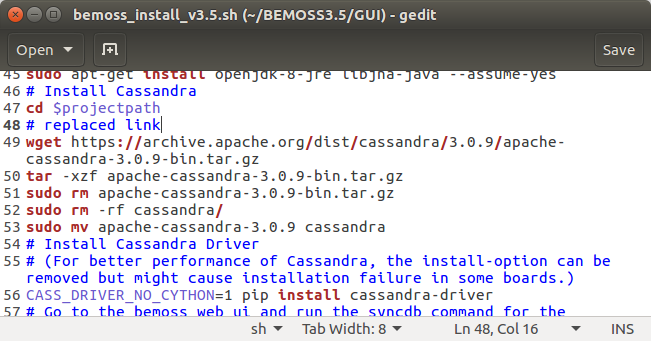
\includegraphics[scale=0.25]{figs/datastaxURLFix.png}
			\end{figure}
		\end{column}
		\begin{column}{0.5\textwidth}
			\begin{block}{Possible Solution}
					Replace http://downloads.datastax.com/
					community/dsc-cassandra-3.0.8-bin.tar.gz with https://archive.apache.org/
					dist/cassandra/3.0.9/apache-cassandra-3.0.9-bin.tar.gz
			\end{block}
		\end{column}
	\end{columns}
\end{frame}

\begin{frame}{Problems}
	\begin{columns}[T]
		\begin{column}{0.5\textwidth}
			\begin{figure}
				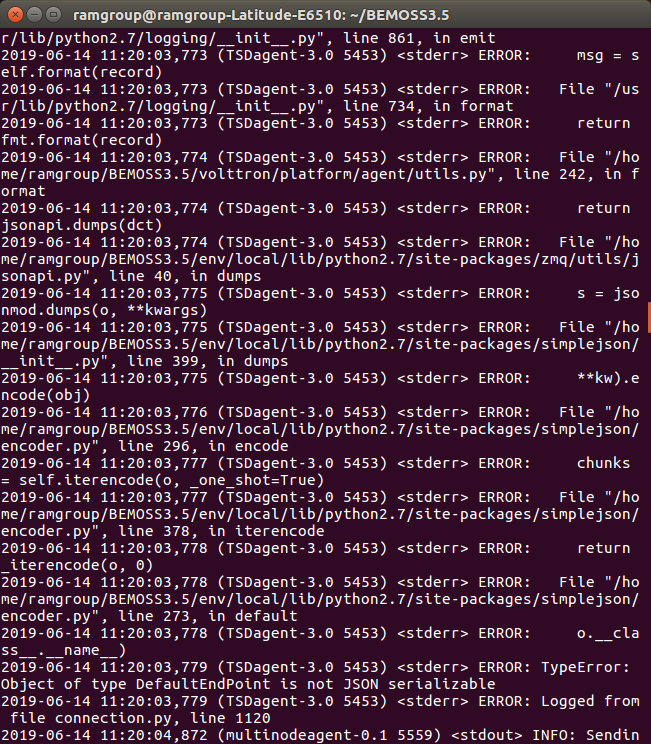
\includegraphics[scale=0.2]{figs/screenshot61419.png}
				\caption{Error raised by BEMOSS during operation}
			\end{figure}
		\end{column}
		\begin{column}{0.5\textwidth}
			\begin{block}{Additional Problems}
				\begin{itemize}
					\item Error reported by TSDagent (Time Series Database Agent) when server is running
					\item Additional changes may need to be made
				\end{itemize}
			\end{block}
		\end{column}
	\end{columns}
\end{frame}

% All of the following is optional and typically not needed. 
%\appendix
%\section<presentation>*{\appendixname}
%\subsection<presentation>*{For Further Reading}

\begin{frame}[allowframebreaks]
  \frametitle<presentation>{Resources}
    
  \begin{thebibliography}{10}
    
  \setbeamertemplate{bibliography item}[online]
  
  \bibitem{bemossinstallation}
    BEMOSS Team
    \newblock BEMOSS Installation Guide
    \newblock \texttt{https://github.com/bemoss/BEMOSS3.5/
    wiki/BEMOSS-Installation-Guide
   } 
  \bibitem{virtualbox}
  	BEMOSS Team
  	\newblock BEMOSS Wiki Images
  	\newblock \texttt{https://github.com/bemoss/wiki\_images/}
 
  \end{thebibliography}
\end{frame}

\end{document}



%%% Local Variables:
%%% mode: latex
%%% TeX-master: t
%%% End:
